\section{Introduction}

\begin{definition}\label{1.1}
    A \emph{(simple) graph}\index{graph} $G$ is a pair $(V, E)$ where $V$ is a non-empty set and $E \subseteq \{\{x,y\} \in V \times V: x \neq y\}$. We call the elements of $V$ \emph{vertices}\index{vertex} of $G$ and the elements of $E$ \emph{edges}\index{edge} of $G$. We also write $V(G)$ for $V$ and $E(G)$ for $E$, respectively.
    
    \lq Simple\rq{} means no loops and no double edges.
\end{definition}

\begin{remark}\label{1.2}
    $V$ is finite, unless otherwise stated.
\end{remark}

\begin{example}\label{1.3}
    We define a few common graphs. Let $n, m \in \mathbb{N}$.
    
    \begin{itemize}

        \item The \emph{complete graph} $K_n$ has $n$ vertices and each pair of vertices is connected.

        \begin{center}
        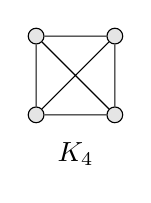
\begin{tikzpicture}[
            vertex/.style={circle, draw, fill=gray!20, minimum size=2mm, inner sep=0pt}
        ]
            \node[vertex] (a) at (0, 1)  {};
            \node[vertex] (b) at (1, 1)  {};
            \node[vertex] (c) at (0, 0)  {};
            \node[vertex] (d) at (1, 0)  {};
            \draw (a)--(b)--(c)--(d)--(a)--(c) (b)--(d);
            \node at (0.5, -0.5) {$K_4$};
        \end{tikzpicture}
        \end{center}

        \item The \emph{cycle} $C_n$ has $n$ vertices, which are cyclically connected.

        \begin{center}
        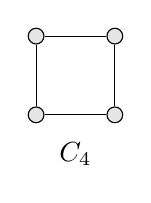
\begin{tikzpicture}[
            vertex/.style={circle, draw, fill=gray!20, minimum size=2mm, inner sep=0pt}
        ]
            \node[vertex] (a) at (0, 1)  {};
            \node[vertex] (b) at (1, 1)  {};
            \node[vertex] (c) at (1, 0)  {};
            \node[vertex] (d) at (0, 0)  {};
            \draw (a)--(b)--(c)--(d)--(a);
            \node at (0.5, -0.5) {$C_4$};
        \end{tikzpicture}
        \end{center}

        \item Let $A$ and $B$ be disjoint sets with $\abs{A} = n$ and $\abs{B} = m$. The \emph{complete bipartite graph} $K_{m,n}$ is defined by
        \begin{align}
            V &= A \dot\cup B\\
            E &= \{\{a, b\}: a \in A, b \in B\}
        \end{align}

        \begin{center}
        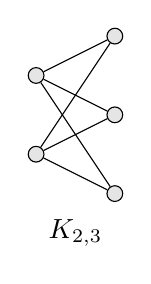
\begin{tikzpicture}[
            vertex/.style={circle, draw, fill=gray!20, minimum size=2mm, inner sep=0pt}
        ]
            \node[vertex] (a1) at (0, 0.5) {};
            \node[vertex] (a2) at (0, 1.5) {};
            \node[vertex] (b1) at (1,   0) {};
            \node[vertex] (b2) at (1,   1) {};
            \node[vertex] (b3) at (1,   2) {};
            \draw (a1)--(b1) (a1)--(b2) (a1)--(b3);
            \draw (a2)--(b1) (a2)--(b2) (a2)--(b3);
            \node at (0.5, -0.5) {$K_{2,3}$};
        \end{tikzpicture}
        \end{center}

        \item The \emph{path} $P_n$ has the vertices $1, \ldots, n$ and edges $\{a, a+1\}$ for $a \in \{1, \ldots, n-1\}$. (in books sometimes $P_{n-1}$ has $n$ vertices)

        \begin{center}
        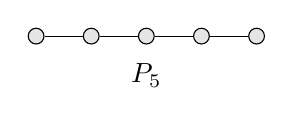
\begin{tikzpicture}[
            vertex/.style={circle, draw, fill=gray!20, minimum size=2mm, inner sep=0pt}
        ]
            \node[vertex] (a) at (0,   0) {};
            \node[vertex] (b) at (0.7, 0) {};
            \node[vertex] (c) at (1.4, 0) {};
            \node[vertex] (d) at (2.1, 0) {};
            \node[vertex] (e) at (2.8, 0) {};
            \draw (a)--(b)--(c)--(d)--(e);
            \node at (1.4, -0.5) {$P_5$};
        \end{tikzpicture}
        \end{center}

    \end{itemize}
\end{example}

\begin{definition}\label{1.4}
    Let $G$ be a graph, $u,v\in V(G)$
    \begin{itemize}
        \item If $\{u,v\}\in E(G)$, then $u$ and $v$ are \textbf{adjacent} and the edge $e=\{u,v\}$ is \textbf{incident} with both $u$ and $v$.
        \item $N_G(v)=\{w\in V(G):\{v,w\}\in E(G)\}$ is the \textbf{neighbourhood} of $v$ in $G$.
        \item $\deg_G(v)=|N_G(v)|$ is the \textbf{degree} of $v$.
    \end{itemize}
\end{definition}

\vspace{0.5cm}

\begin{lemma}[Handshake Lemma]\label{1.5}
    Let $G$ be a graph. Then
    \begin{align}
        \sum\limits_{v \in V(G)} \deg_G(v) = 2 \abs{E(G)}.
    \end{align}
    (in particular the sum of the degree is even).
    
    \begin{proof}
        $\sum\limits_{v\in V(G)} \deg_G(v)=\#\{(v,e):v\in V(G),e\in E(G) \text{ such that } v \text{ incident to } e \}=2|E(G)|$
    \end{proof}
\end{lemma}

\vspace{0.5cm}

\begin{definition}\label{1.6}
    Two graphs $G=(V,E)$ and $G'=(V',E')$ are \textbf{isomorphic} if there exists an isomorphism $\phi$ between them, i.e. a bijection $\phi:V\to V'$ such that $\forall u,v\in V(G):\{u,v\}\in E(G)\iff \{\phi(u),\phi(v)\}\in E(G')$
\end{definition}

\vspace{0.5cm}

\begin{definition}\label{1.7}
    Let $G=(V,E)$ be a graph. A \textbf{subgraph} of $G$ is a graph $H=(V',E')$ with $V'\subseteq V$ and $E'\subseteq E\cap \begin{pmatrix} V' \\ 2 \end{pmatrix}$ where $\begin{pmatrix}
        S \\ K
    \end{pmatrix}$ is the set of all $K$-subsets of $S$.\par
    $H'$ is an \textbf{induced subgraph} of $G$ if it is a subgraph and $E'=E\cap \begin{pmatrix}
        V' \\ 2
    \end{pmatrix}$\par
    $H''$ is a \textbf{spanning subgraph} if it is a subgraph and $V'=V$\par
    For $W\subseteq V$, write $G[W]$ for the subgraph induced by the vertices in $W$
\end{definition}
\begin{example}\label{1.8}
\hfill
    \begin{center}
        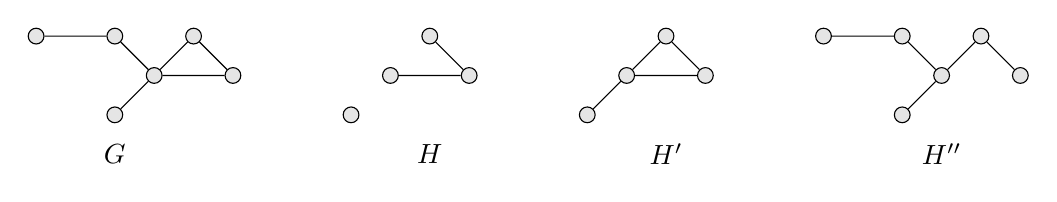
\begin{tikzpicture}[
            vertex/.style={circle, draw, fill=gray!20, minimum size=2mm, inner sep=0pt}
        ]
            \node[vertex] (a) at (-6,   1) {};
            \node[vertex] (b) at (-5, 1) {};
            \node[vertex] (c) at (-4.5, 0.5) {};
            \node[vertex] (d) at (-5, 0) {};
            \node[vertex] (e) at (-4, 1) {};
            \node[vertex] (f) at (-3.5,0.5){};
            \draw (a)--(b)--(c)--(d);
            \draw (c)--(e)--(f)--(c);
            \node at (-5, -0.5) {$G$};

            \node[vertex] (c') at (-1.5, 0.5) {};
            \node[vertex] (d') at (-2, 0) {};
            \node[vertex] (e') at (-1, 1) {};
            \node[vertex] (f') at (-0.5,0.5){};
            \draw (e')--(f')--(c');
            \node at (-1, -0.5) {$H$};

            \node[vertex] (c'') at (1.5, 0.5) {};
            \node[vertex] (d'') at (1, 0) {};
            \node[vertex] (e'') at (2, 1) {};
            \node[vertex] (f'') at (2.5,0.5){};
            \draw (e'')--(f'')--(c'')--(e'');
            \draw (c'')--(d'');
            \node at (2, -0.5) {$H'$};

            \node[vertex] (a''') at (4,   1) {};
            \node[vertex] (b''') at (5, 1) {};
            \node[vertex] (c''') at (5.5, 0.5) {};
            \node[vertex] (d''') at (5, 0) {};
            \node[vertex] (e''') at (6, 1) {};
            \node[vertex] (f''') at (6.5,0.5){};
            \draw (a''')--(b''')--(c''')--(d''');
            \draw (c''')--(e''')--(f''');
            \node at (5.5, -0.5) {$H''$};
        \end{tikzpicture}
        \end{center}
\end{example}

\vspace{1cm}

\begin{definition}\label{1.9}
Let $v_i$ be vertices of a graph $G$
    \begin{itemize}
        \item A \textbf{walk} is a sequence of vertices $v_i$ s.t. $\{v_i,v_{i+1}\}\in E(G) \forall i\in \{1,...,k-1\}$
        \item The \textbf{length} of a walk is $k$ (number of vertices in the walk)
        \item The walk is \textbf{closed} if $v_1=v_k$
        \item A \textbf{trail} is a walk that does not use an edge twice
        \item A \textbf{path} is a walk for which $v_1,...,v_k$ are pairwise distinct
    \end{itemize}
    \begin{center}
        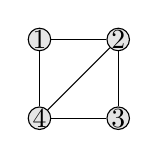
\begin{tikzpicture}[
            vertex/.style={circle, draw, fill=gray!20, minimum size=2mm, inner sep=0pt}
        ]
            \node[vertex] (a) at (0, 0) {$4$};
            \node[vertex] (b) at (0, 1) {$1$};
            \node[vertex] (c) at (1, 1) {$2$};
            \node[vertex] (d) at (1, 0) {$3$};
            \draw (a)--(b)--(c)--(d)--(a);
            \draw (a)--(c);
            \node at (0.5, 0.5) {};

        \end{tikzpicture}
        \end{center}
        $(1,2,3,4,2,3)$ is a walk, but no trail \\
        $(1,2,3,4,2)$ is a trail, no path \\
        $(1,2,3,4)$ is a path
\end{definition}

\vspace{0.5cm}

\begin{definition} \label{1.10}
Let $G$ be a graph
    \begin{itemize}
        \item A graph $G$ is \textbf{connected} if there is a walk between any pair of its vertices
        \item A \textbf{(connected) component} of $G$ is an inclusion wise maximal connected subgraph
    \end{itemize}
\end{definition}


\subsection{Hamiltonian Cycles}

\begin{definition}\label{1.11}
    A \textbf{Hamiltonian cycle}\index{Hamiltonian cycle} in a graph $G$ is a spanning subgraph that is a cycle (isomorphic to $C_n$ for some $n\in\mathbb{N}$)\\
    If $G$ has a Hamiltonian cycle, $G$ is called \textbf{Hamiltonian} 
\end{definition}

\vspace{0.5cm}

\begin{theorem}[Dirac's Theorem]\label{1.12}
    Let $G$ be a graph of order $n\geq 3$ where the \textbf{order}\index{order} of $G$ is given by $|V(G)|$ and the \textbf{size} by $|E(G)|$. If every Vertex of $G$ has degree at least $\frac{n}{2}$ then $G$ is Hamiltonian 
\end{theorem}

\vspace{0.5cm}

\begin{theorem}[Ore's theorem]\label{1.13}
    Let $G$ be a graph of order $n\geq3$. If for every pair $u,v\in V,u\neq v,u$ and $v$ non-adjacent, we have $\deg(u)+\deg(v)\geq n$ then $G$ is Hamiltonian
\end{theorem}
\begin{remark}\label{1.14}
\hfill \\
    Ore $\implies$ Dirac
\end{remark}
\begin{proof}
    \begin{itemize}
    \hfill \\
        \item The Graph $G$ is connected: suppose $G$ is not connected. Take an arbitrary component of $G$ and call it $H$. The order of $H$ is $n-k$ if $k$ vertices are not in $V(H)$. Now any $v\in V(H)$ has $\deg(v)\leq n-k-1$ with equality if $v$ is adjacent to every vertex in $V(H)$. Now take $u\notin V(H)$ so $\deg(u)\leq k-1$. It follows that $u,v\in V(G),u\neq v$ and $u,v$ are not adjacent so $\deg(u)+\deg(v)\geq n$ but $\deg(u)+\deg(v)\leq k-1+n-k-1=n-2<n$ $\lightning$
        \item $G$ has a Hamiltonian cycle: By induction on the number of non-edges
        \item No non-edge $\implies G$ complete, hence Hamiltonian
        \item Assume $G$ non complete $u,v\in V, u\neq v$, be non-adjacent. By induction the graph $G'$ obtained from $G$ by adding $e=\{u,v\}$ as an edge is Hamiltonian. Let~$C$ be a Hamiltonian cycle of $G'$. If $C$ does not use $e\implies C$ is Hamiltonian cycle in $G$. Assume $C$ uses $e$. Removing $e$ from $C$ yields a path from $u$ to $v$\par
        For $i\in\{2,...,n-1\}$
        \item If $v_i$ is a neighbour of $u$, color $\{v_{i-1},v_i\}$ red
        \item If $v_i$ is a neighbour of $v$, color $\{v_{i},v_{i+1}\}$ blue
        \item Since $\deg(u)+\deg(v)\geq n$ and the path $v_1,...,v_n$ has $n-1$ edges, there exists an edge $\{v_{i},v_{i+1}\}$ which is both red and blue. Then $v_1,...v_i,v_n,v_{n-1},...,v_{i+1}$ is a Hamiltonian cycle in $G$.
    \end{itemize}
    \begin{center}
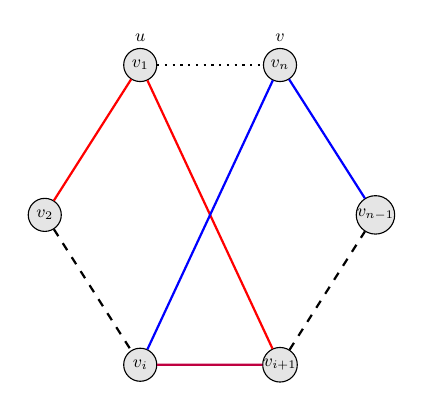
\begin{tikzpicture}[ scale=0.7,
    vertex/.style={circle, draw, fill=gray!20, minimum size=6mm, inner sep=0pt},
    every node/.style={font=\small, transform shape}
]
\def\r{3}
\node[vertex] (v1)  at ({90-335}:\r)            {$v_1$};
\node[vertex] (vn)  at ({90-25}:\r)         {$v_n$};
\node[vertex] (vi)  at ({90-205}:\r)        {$v_i$};
\node[vertex] (vi1) at ({90-155}:\r)        {$v_{i+1}$};
\node[vertex] (v2) at ({90-270}:\r)        {$v_2$};
\node[vertex] (vn1)  at ({0}:\r)        {$v_{n-1}$};

\draw[thick, red] (v1)--(v2);
\draw[thick, blue] (vn)--(vn1);
\draw[thick, dotted] (v1)--(vn);
\draw[thick, dashed] (v2)--(vi);
\draw[thick, dashed] (vi1)--(vn1);
\draw[thick, purple] (vi)--(vi1); 
\draw[thick, red] (v1)--(vi1);
\draw[thick, blue] (vn)--(vi);

% Labels for u and v
\node[above=3mm] at (v1)  {$u$};
\node[above=3mm]  at (vn)  {$v$};

\end{tikzpicture}
\end{center}
\end{proof}
\subsection{EulerianTrail}

\begin{definition}
    An \textbf{Eulerian trail} is a trail that passes through each edge of the graph exactly once. A graph with a closed Eulerian trail is called \textbf{Eulerian}
\end{definition}
\vspace{0.5cm}
\begin{theorem}[Euler's theorem]
    Let $G$ be a connected graph with at least 2 vertices. Then $G$ has a closed Eulerian trail iff every vertex in G has even degree
\end{theorem}
\begin{proof}
\hfill \\
    "$\implies$" \\
    Let $T$ be a closed Eulerian trail and fix an orientation on $T$. Then for every $v\in V(G)$, the incident edges can be classified as "ingoing" or "outgoing". This defines a bijection between in and outgoing edges of $T$, so $\deg(v)$ is even.\\
    "$\impliedby$" \\
    Let $T=(v_0,e_1,v_1,...,e_m,v_m)$ be a longest trail. We will prove (i) $v_0=v_m$ and (ii) $\{e_i:i\in \{1,...,m\}\}=E(G)$. (i)$+$(ii)$\iff T$ is closed Eulerian trail.\\
    \begin{enumerate}
        \item If $v_0\neq v_m$, then $v_0$ is incident to an odd number of edges in $T$. As $\deg(v_0)$ is even, there is $e\in E(G)$ incident to $v_0$ and not on $T$. We could thus append $e$ on $T$ $\lightning$ because $T$ is longest trail.
        \item Claim: $V(T)=V$. Assume otherwise there exists a vertex $v'\notin V(T)$ and $e=\{v_k,v'\}\in E(G)$ for some $k\in \{0,...,m\}$ (by connectedness). Then $(v',e,v_k,e_{k+1},v_{k+1},...,v_{m-1},e_m,v_0,e_1,...,v_{k-1},e_k)$ is a longer trail hence $V(T)=V$
        \begin{center}
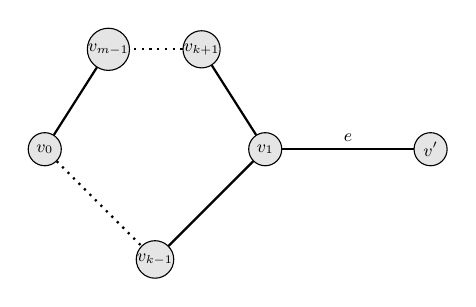
\begin{tikzpicture}[ scale=0.7,
    vertex/.style={circle, draw, fill=gray!20, minimum size=6mm, inner sep=0pt},
    every node/.style={font=\small, transform shape}
]
\def\r{2}
\node[vertex] (v1)  at ({90-335}:\r)   {$v_{m-1}$};
\node[vertex] (vm)  at ({90-25}:\r)    {$v_{k+1}$};
\node[vertex] (v2) at ({90-270}:\r)    {$v_0$};
\node[vertex] (vk)  at ({0}:\r)        {$v_1$};
\node[vertex] (vp) at (5, 0) {$v'$};
\node[vertex] (vk1) at ({-90}:\r) {$v_{k-1}$};

\draw[thick] (vk) -- node[midway, above] {$e$} (vp);
\draw[thick] (vk)--(vm);
\draw[thick] (v1)--(v2);
\draw[thick] (vk)--(vk1);
\draw[thick, dotted] (v2)--(vk1);
\draw[thick, dotted] (vm)--(v1);
\end{tikzpicture}
\end{center}
\par
        Claim: $E(T)=E$. Assume otherwise. Consider $e\in E\setminus E(1)$ and write $e=\{v_k,v_l\}$. Then $(v_k,e_{k+1},v_{k+1},...,v_{m-1},e_m,v_0,e_1,v_1,...,e_k,v_k,e,v_l)$ is a longer trail $\lightning$ 
    \end{enumerate}
\end{proof}
\vspace{0.5cm}

\begin{theorem}
    Let $G$ be a connected graph with at least two vertices. Then $G$ has an Eulerian trail iff there are precisely $0$ or two vetices of odd degree
\end{theorem}
\begin{proof}
    \hfill\\
    By the Euler's Theorem, we know that if there are $0$ vertices of odd degree then there exists an Eulerian trail (in fact a closed Eulerian trail), and if there exists a closed Eulerian trail, then all vertices have even degree.\par
    Suppose now that $G$ has exactly two vertices $x$ and $y$ of odd degree. We consider the following graph $G'$: Set $V(G')=V(G)\cup \{z\}$, where $z\notin V(G)$. Furthermore set $E(G')=E(G)\cup\{\{x,z\},\{y,z\}\}$. Clearly, every vertex has even degree in $G'$, so there exists a closed Eulerian trail. Since $z$ is only adjacent to $x$ and $y$, these are the neighbours of $z$ on the trail. Deleting the edges $\{x,z\}$ and $\{y,x\}$ from the trail yields an Eulerian trail from $x$ to $y$ in $G$. Conversely, if there is a non-closed Eulerian trail with endpoints $x$ and $y$ in $G$, then $x$ and $y$ are non-adjacent. Adding the edge $\{x,y\}$ creates a graph with a closed Eulerian trail, so all vertices have even degree by Euler's theorem. Thus $x$ and $y$ are the only verices in $G$ with odd degree.
\end{proof}
\subsection{Datastructures}

Assume that $G=(V,E)$ is a graph with $v=\{1,...n\}$
\vspace{0.5cm}
\begin{definition}\label{1.18}
    The \textbf{adjacency matrix} of $G$ is the matrix $A=(a_{ij})$ with $a_{ij}=\begin{cases}
            1 & \{i,j\}\in E \\
            0 & else
            \end{cases}$\\
    The \textbf{adjacency list} of $G$ stores a label for each vertex, and a list of (pointers to) its neighbours.
\end{definition}
\begin{example}\label{1.19}
\hfill \\
        \begin{center}
        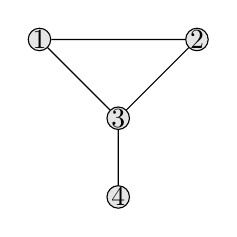
\begin{tikzpicture}[vertex/.style={circle, draw, fill=gray!20, minimum size=2mm, inner sep=0pt}]
        \node[vertex] (v1)  at (-1,2) {$1$};
        \node[vertex] (v2)  at (1,2)  {$2$};
        \node[vertex] (v3)  at (0,1)  {$3$};
        \node[vertex] (v4)  at (0,0)  {$4$};

        \draw (v4)--(v3)--(v1)--(v2)--(v3);
        \end{tikzpicture}
        \end{center}
        $A=
        \begin{pmatrix}
        0 & 1 & 0 & 1 \\
        1 & 0 & 1 & 1 \\
        0 & 1 & 0 & 0 \\
        1 & 1 & 0 & 0
        \end{pmatrix}$
        \begin{itemize}
            \item $v_1$: $v_2, v_4$
            \item $v_2$: $v_1, v_3, v_4$
            \item $v_3$: $v_2$
            \item $v_4$: $v_1, v_2$
        \end{itemize}
\end{example}
\vspace{0.5cm}

\begin{remark}\label{1.20}
\hfill \\
    Memory requirement: \par
    Adjacency matrix: $\theta (n^2)$\par
    Adjacency list: $\theta (n+m)$, where $m$ is the number of edges
\end{remark}